% Please do not change the document class
\documentclass{scrartcl}

% Please do not change these packages
\usepackage[hidelinks]{hyperref}
\usepackage[none]{hyphenat}
\usepackage{setspace}
\usepackage{graphicx}
\usepackage{subcaption}
\doublespace

% You may add additional packages here
\usepackage{amsmath}

% Please include a clear, concise, and descriptive title
\title{COMP210 - Research Journal}

% Please put your student number in the author field
\author{1507729}

\begin{document}

\maketitle

\section{Putting Man above Motion}

Virtual reality (VR) isn't a new idea, with some even claiming it's been around since the 1950s. \cite{vrs2017origin} There have been many attempts at getting VR into the public however each time the technology to support VR hasn't been able to keep up. While developments happen in VR technology it's popularity has grown within the gaming community however recent VR devices can cause users to feel ill for a number of reasons. \cite{porcino2017minimizing} The term used is called cyber sickness though it's also been called simulator sickness \cite{gower1989simulator} previously.

\begin{figure}[h!]

\centering

\begin{subfigure}[b]{0.3\linewidth}
	\centering
	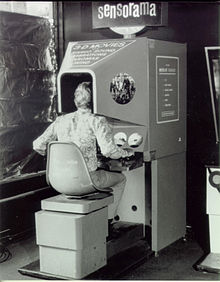
\includegraphics[width=\linewidth]{Sensorama.jpg}
	\caption{Sensorama}
\end{subfigure}%
~
\begin{subfigure}[b]{0.3\linewidth}
	\centering
	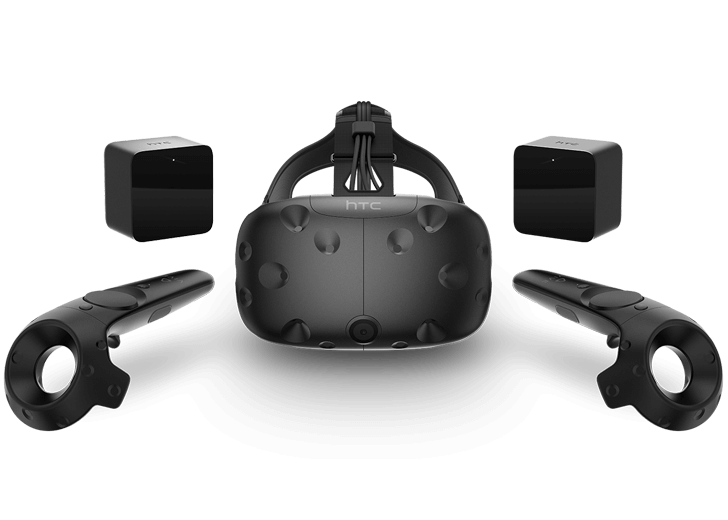
\includegraphics[width=\linewidth]{vive.png}
	\caption{HTC Vive}
\end{subfigure}
\caption{An comparison of earlier and modern VR equipment.}
\label{fig:VR}

\end{figure}

\bibliographystyle{ieeetran}
\bibliography{references}

\end{document}
